%!TEX root = ../main.tex

\chapter{Einleitung} % (fold)
% \addcontentsline{toc}{chapter}{Einleitung}
\label{cha:einleitung}

\section{Motivation} % (fold)
\label{sec:motivation}

Ein Polymer, oder auch Makromolekül, ist ein Molekül, welches sich aus vielen kleineren, sich wiederholenden Molekülen, sogenannten Monomeren, zusammensetzt.
Besteht ein Polymer aus nur einer Monomer-Art, dann spricht man von einem Homopolymer, sonst von einem Heteropolymer oder auch Copolymer.
Typischerweise besteht ein Polymer aus einer langen Kette von aneinanderhängenden Monomeren, es existieren aber auch weitere Konfigurationen, zum Beispiel stern- oder ringförmige Anordnungen.

Copolymere lassen sich anhand der Anordnung der Monomere weiter klassifizieren.
Bilden die verschiedenen Monomer-Gattungen homogene, zusammenhängede Gruppen, welche wiederum durch aneinanderreihen das Copolymer bilden, dann nennen wir dies ein Blockcopolymer, vergleiche \autoref{fig:konfig}.

Es existieren unüberschaubar viele solcher Konfigurationen von Polymeren, und insbesondere Blockcopolymeren, weswegen man häufig auf das Studium vergleichsweise simpler Anordnungen zurückgreift.
Als besonders beliebt hat sich der Fall des kettenförmigen Blockcopolymers mit zwei Monomer-Typen, der Einfachheit halber A und B genannt, herausgestellt.
Diese Konfiguration wird auch als AB-Diblockcopolymer bezeichnet.

\begin{figure}[tb]
    \centering
    \begin{subfigure}[b]{\textwidth}
        \centering
        \includestandalone[width=0.8\textwidth]{tikz/einleitung/fig1}
    \end{subfigure}
    \\[1em]
    \begin{subfigure}[b]{\textwidth}
        \centering
        \includestandalone[width=0.8\textwidth]{tikz/einleitung/fig2}
    \end{subfigure}
    \\[1em]
    \begin{subfigure}[b]{\textwidth}
        \centering
        \includestandalone[width=0.8\textwidth]{tikz/einleitung/fig3}
    \end{subfigure}
    \caption[Skizzenhafte Darstellung verschiedener Polymerarten]{%
        Skizzenhafte Darstellung verschiedener Polymerarten.
        Von oben nach unten: Homopolymer, ein AB-Diblockcopolymer und ein sogenanntes statistisches AB-Copolymer, bei dem die beiden Monomer-Arten zufällig verteilt sind.
    }
    \label{fig:konfig}
\end{figure}

Von großem Interesse ist das Verhalten von Polymerschmelzen, das heißt, des flüssigen Aggregatzustands eines Polymers, sowie das Verhalten von Gemischen verschiedener polymerer Stoffe.
So neigen die Gemische vieler Paare von Homopolymeren zu makroskopischer Phasenseparation, wie man es zum Beispiel von Öl und Essig kennt.
Eine ähnliche Tendenz findet man auch bei den Polymerschmelzen von Blockcopolymeren, hierbei kann aufgrund der Verbindung der verschiedenen Monomer-Blöcke aber keine makroskopische Phasenseparation auftreten.
Stattdessen kommt es zu einer periodischen, mikroskopischen Separation.
\autoref{fig:anordnungen} zeigt einige mögliche Anordnungen, die bei Diblockcopolymeren tatsächlich experimentell beobachtet wurden.

\begin{figure}[tb]
    \centering
    \begin{subfigure}[b]{0.18\textwidth}
        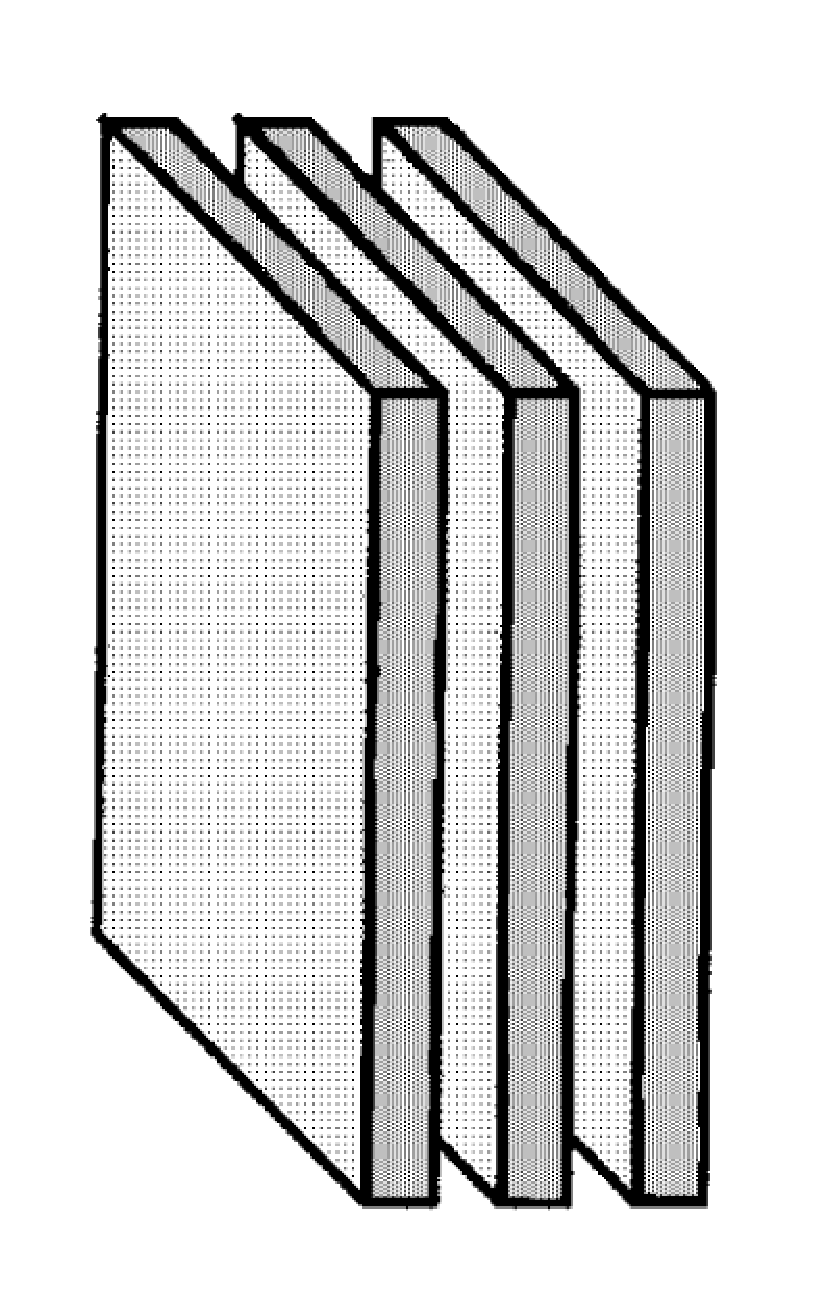
\includegraphics[width=\textwidth]{figures/einleitung/fig1}
    \end{subfigure}
    \begin{subfigure}[b]{0.18\textwidth}
        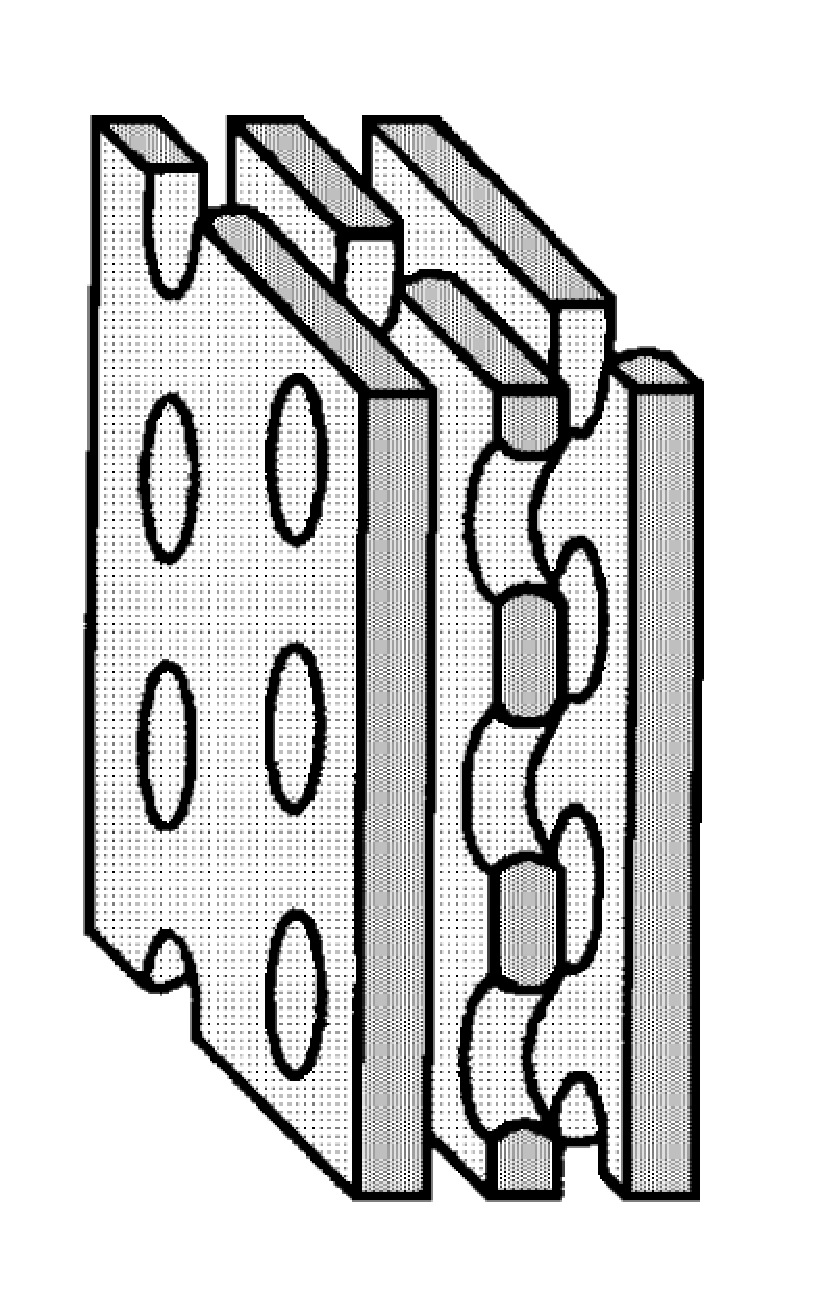
\includegraphics[width=\textwidth]{figures/einleitung/fig2}
    \end{subfigure}
    \begin{subfigure}[b]{0.18\textwidth}
        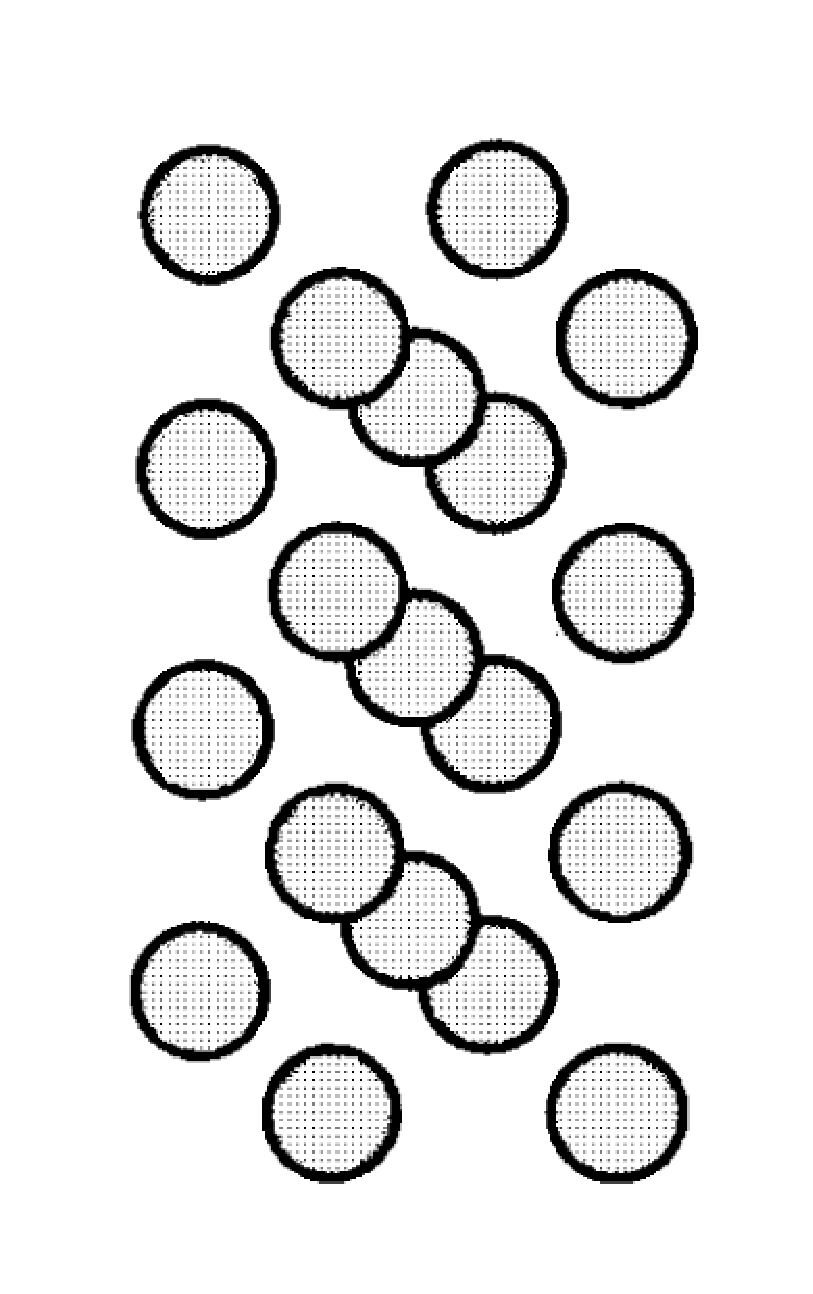
\includegraphics[width=\textwidth]{figures/einleitung/fig3}
    \end{subfigure}
    \begin{subfigure}[b]{0.18\textwidth}
        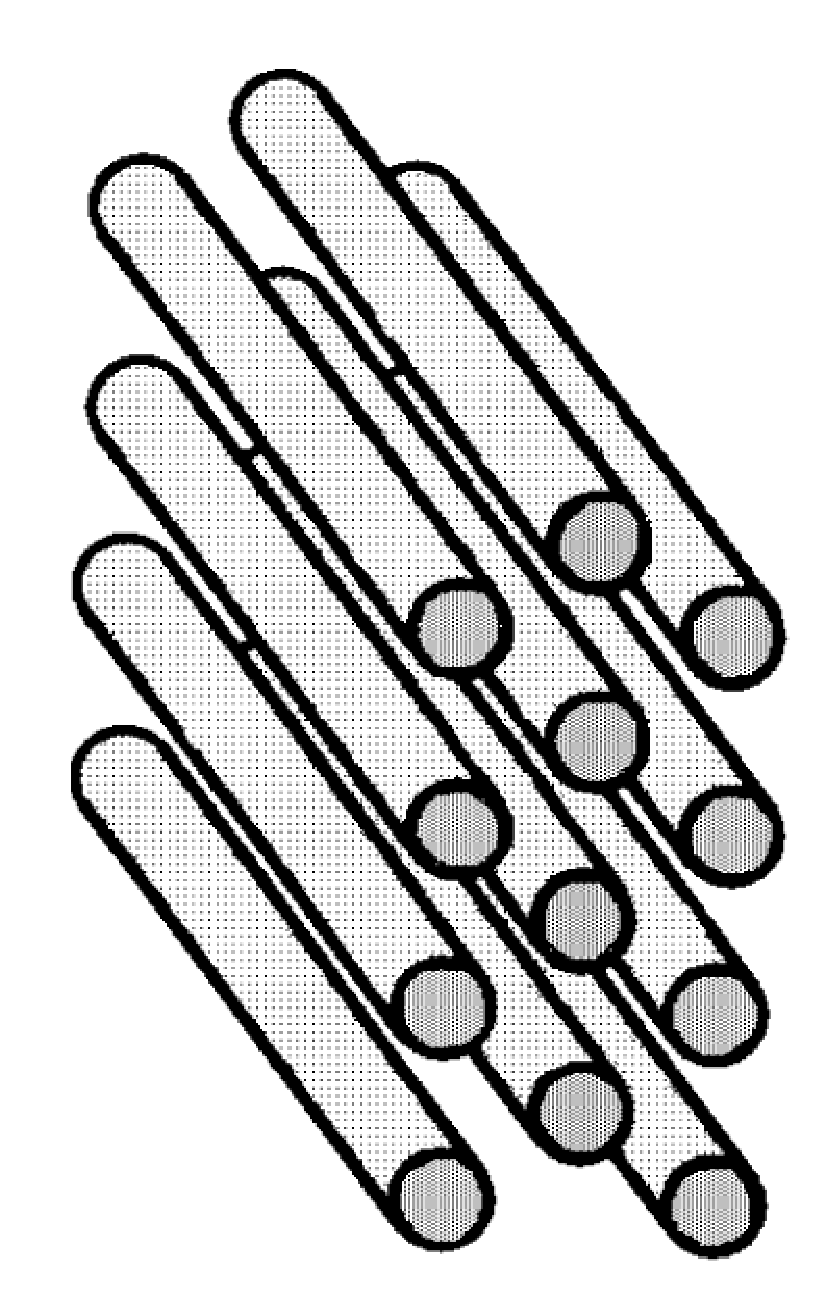
\includegraphics[width=\textwidth]{figures/einleitung/fig4}
    \end{subfigure}
    \begin{subfigure}[b]{0.18\textwidth}
        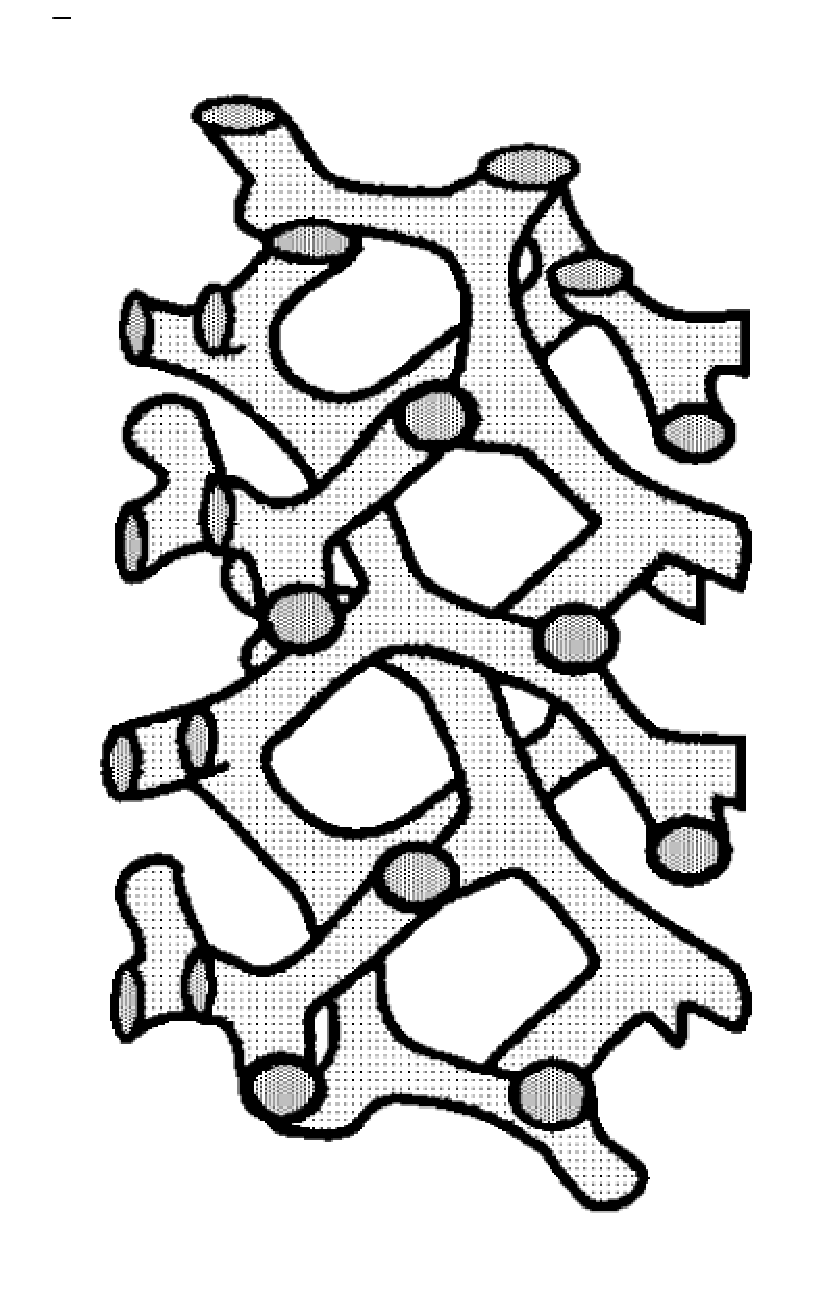
\includegraphics[width=\textwidth]{figures/einleitung/fig5}
    \end{subfigure}
    \caption[Verschiedene Phasen bei Diblockcopolymeren]{%
        Verschiedene Phasen bei Diblockcopolymeren, welche experimentell beobachtet wurden, wobei hierbei nur eine der beiden Monomer-Gattungen dargestellt wird.
        Diese heißen von links nach rechts: Lamellar, Perforiert-Lamellar, Sphärisch, Zylindrisch, Gyroid.
        Diese Abbildung wurde \cite[Figure 1.18]{Matsen:2006ud} entnommen.
    }
    \label{fig:anordnungen}
\end{figure}

Da die experimentelle Bestimmung ohne Vorwissen über die möglichen, stabilen Anordnungen nur wenig erfolgversprechend ist, wird eine fundierte Theorie benötigt, auf Basis derer theoretische Vorhersagen getroffen werden können, die vorzugsweise wiederum experimentell belegbar sein sollten.
Da Diblockcopolymere einen relativ simplen Fall eines Copolymers darstellen, wurde sowohl in die experimentelle als auch theoretische Untersuchung dieser bereits vergleichsweise viel Arbeit investiert.

Als besonders nützliche und dennoch relativ einfache Theorie hat sich das auf der sogenannten selbstkonsistenten Feldtheorie, im Weiteren wird der englische Ausdruck \emph{self-consistent field theory}, kurz SCFT, verwendet, basierende Modell herausgestellt.

\paragraph{Self-consistent field theory} % (fold)
\label{par:self_consistent_field_theory}

Die self-consistent field theory ist ein weit verbreitetes theoretisches Modell der Physik um das Verhalten von Teilchen unter Einwirkung von Kräften, die durch Wechselwirkung mit anderen Teilchen auftreten, zu studieren.
Mit Hilfe dieses Modells lässt sich die statistische räumliche Verteilung eines Teilchens bestimmen.
Hierbei wird zur Vereinfachung des Modells das eigentlich vorliegende Mehrkörperproblem durch mitteln der Wechselwirkungen auf ein Einkörperproblem reduziert.

Für den Fall von Diblockcopolymeren lässt sich das resultierende Modell folgendermaßen zusammenfassen.

Betrachte den Fall einer inkompressiblen Polymerschmelze linearer AB-Diblockcopolymere.
Der Einfachheit halber bestehe jede solche Polymerkette aus insgesamt $N = N_{A} + N_{B}$ Monomeren, wobei $N_{A}$ die Anzahl der $A$-Monomere und $N_{B}$ dementsprechend die Anzahl der $B$-Monomere einer Polymerkette sei.
Weiter bezeichnen wir mit $f = \frac{N_{A}}{N}$ den Anteil der $A$-Monomere an der Gesamtzahl der vorkommenden Monomere.
Bezeichne $s$ eine Distanz entlang der Polymerkontur, so normalisiert, dass $0 \leq s \leq 1$, wobei $0$ und $1$ den beiden Enden des Polymers entsprechen.
Wir gehen von gleicher \emph{statistischer Länge} $a$ für die beiden Monomer-Typen aus und von einer \emph{uniform segment concentration} $\rho_{0}$.
Damit ergibt sich das Gesamtvolumen der Polymerschmelze zu $V = \frac{nN}{\rho_{0}}$ und wir bezeichnen mit $\vec{r}$ eine Position in diesem System.
Wir können nun die Konzentration eines Monomers vom Typ $\alpha \in \Set{A, B}$ an einem Punkt $\vec{r}$ durch eine Funktion $\phi_{\alpha}(\vec{r})$ angeben.

Da es sich bei dem betrachteten Fall um eine inkompressible Schmelze handelt,
liefert dies die notwendige Bedingung
\begin{equation}
\label{eq:einleitung:inkompressible}
    \phi_{A}(\vec{r}) + \phi_{B}(\vec{r}) = 1
\end{equation}
für jeden Punkt $\vec{r}$ im betrachteten System.

Bei der self-consistent field theory wird das Mehrkörperproblem der Wechselwirkungen zwischen den Polymeren umgangen, indem die einzelnen Polymerketten als Random Walk, der durch ein \emph{chemical potential field} gesteuert wird, interpretiert werden.

Diese Felder werden approximiert durch
\begin{equation}
\label{eq:einleitung:felder}
    \begin{aligned}
        \omega_{A}(\vec{r}) = \chi N \phi_{B}(\vec{r}) + \xi(\vec{r}),\\
        \omega_{B}(\vec{r}) = \chi N \phi_{A}(\vec{r}) + \xi(\vec{r}),
    \end{aligned}
\end{equation}
wobei $\chi$ der sogenannte Flory-Huggins-Wechselwirkungsparameter für die Wechselwirkungen zwischen den Monomeren vom Typ $A$ und $B$ ist und $\xi(\vec{r})$ ein Lagrange-Multiplikator ist, welcher die Inkompressibilität \eqref{eq:einleitung:inkompressible} erzwingen soll.

\todo[inline]{Gelaber}

Dies führt auf die parabolischen partiellen Differentialgleichung
\begin{equation}
\label{eq:einleitung:mde}
    \begin{aligned}
        \frac{\partial q}{\partial s}(\vec{r}, s) &= \frac{N a^{2}}{6} \Delta_{\vec{r}} q(\vec{r}, s) - \omega_{\alpha(s)}(\vec{r}) q(\vec{r}, s),\\
        -\frac{\partial q^{\dagger}}{\partial s}(\vec{r}, s) &= \frac{N a^{2}}{6} \Delta_{\vec{r}} q^{\dagger}(\vec{r}, s) - \omega_{\alpha(s)}(\vec{r}) q^{\dagger}(\vec{r}, s)
    \end{aligned}
\end{equation}
mit den Anfangsbedingungen $q(\vec{r}, 0) = q^{\dagger}(\vec{r}, 1) = 1$.

Die Felder $\omega_{\alpha(s)}$ sind dabei gegeben durch
\begin{equation}
    \omega_{\alpha(s)}(\vec{r}) = \begin{cases}
        \omega_{A}(\vec{r}), & 0 \leq s \leq f\\
        \omega_{B}(\vec{r}), & f < s \leq 1.
    \end{cases}
\end{equation}

Hat man die Lösungen dieser Differentialgleichung bestimmt, dann können die Anteile der Monomere berechnet werden über

\begin{equation}
    \begin{aligned}
        \phi_{A}(\vec{r}) = \frac{1}{Q} \int_{0}^{f} q(\vec{r}, s) q^{\dagger}(\vec{r}, s) \diff s,\\
        \phi_{B}(\vec{r}) = \frac{1}{Q} \int_{f}^{1} q(\vec{r}, s) q^{\dagger}(\vec{r}, s) \diff s,
    \end{aligned}
\end{equation}
wobei $Q$ ein Normalisierungsfaktor ist, der durch
\begin{equation}
    Q = \frac{1}{V} \int q(\vec{r}, 1) \diff \vec{r}
\end{equation}
gegeben ist.

Ist eine selbstkonsistente Lösung gefunden, dann lässt sich die freie Energie einer Polymerkette in der resultierenden Anordnung berechnen via
\begin{equation}
\label{eq:einleitung:freie_energie}
    \frac{F}{n k_{B} T} = - \ln(\frac{Q}{V}) + \frac{1}{V} \int \chi N \phi_{A}(\vec{r}) \phi_{B}(\vec{r}) \diff \vec{r} - \frac{1}{V} \int \omega_{A}(\vec{r}) \phi_{A}(\vec{r}) + \omega_{B}(\vec{r}) \phi_{B}(\vec{r}) \diff \vec{r}.
\end{equation}

\section{Einsatz numerischer Methoden} % (fold)
\label{sec:bisherige_numerische_methoden}

Unter Verwendung des theoretischen Grundgerüsts der selbstkonsistenten Feldtheorie aus dem vorherigen Abschnitt lassen sich numerische Iterationsverfahren konstruieren, mit denen stabile Anordnungen von Polymerketten in der Schmelze eines Diblockcopolymers bestimmt werden können.
Dazu wird ein Sattelpunkt des Funktionals der freien Energie \eqref{eq:einleitung:freie_energie} gesucht.
Dieser muss nicht eindeutig sein.
Wie aus dem vorherigen Abschnitt bekannt ist, erfüllt ein solcher Sattelpunkt gerade die Inkompressibilität \eqref{eq:einleitung:inkompressible} und weiter die Bedingung \eqref{}.
Diese beiden Gleichungen lassen sich ausnutzen um ein Newton-artiges Iterationsverfahren zu konstruieren.
Dabei stellen sich die folgenden beiden Punkte als besonders wichtig heraus, da sie massiv die Laufzeit des Iterationsverfahren beeinflussen.
Von besonderer Bedeutung sind daher:
\begin{enumerate}
    \item das Lösungsverfahren für die parabolischen partiellen Differentialgleichung \eqref{eq:einleitung:mde},
    \item das \emph{Mixing}-Verfahren, mit dem iterativ die neuen Konzentrationen $\phi_{A}, \phi_{B}$ und zugehörigen Felder $\omega_{A}, \omega_{B}$ bestimmt werden.
\end{enumerate}

Auf den zweiten Punkt, das Mixing-Verfahren, werden wir im weiteren Verlauf dieser Arbeit nicht weiter eingehen.
Trotz dessen, und insbesondere, da es viele, sehr verschiedene Verfahren gibt, die hierfür zum Einsatz kommen, wollen wir hier einige Ansätze nennen.
Da es sich beim Mixing-Schritt im Wesentlichen um die Suche nach einem Sattelpunkt eines nichtlinearen Funktionals handelt, lassen sich hierfür viele bekannte Verfahren der nichtlinearen Optimierung, aber auch aus anderen Bereichen, anwenden.

Dies reicht von einem Quasi-Newton-Verfahren bei \textcite{Matsen:1994bz}, welches direkt an den darin verwendeten Löser für die partielle Differentialgleichung \eqref{eq:einleitung:mde} gekoppelt ist, bis zu Integrationsverfahren, wie zum Beispiel Runge-Kutta-Verfahren oder Mehrschrittverfahren.
Ein auf einem solchen Integrationsverfahren basierendes Mixing, neben einem weiteren, welches auf einem Conjugated-Gradients-Verfahren aufbaut, findet sich bei \textcite{Ceniceros:2006is}.
Als besonders nützlicher Ansatz hat sich das sogenannte Anderson-Mixing erwiesen, siehe die Arbeiten von \textcite{Thompson:2004um,Stasiak:2011ba}.
Dabei werden neue Felder durch Kombination der Felder vieler zurückliegender Iterationen gewonnen.
Ein weiteres, einer Picard-Iteration ähnliches, Verfahren findet man bei \textcite{Drolet:1999bs}.

Unser Hauptaugenmerk in dieser Arbeit liegt auf dem ersten Punkt, dem wiederholten Lösen der parabolischen partiellen Differentialgleichung \eqref{eq:einleitung:mde}.
Da es, abhängig vom gewählten Mixing-Verfahren, oftmals eine Iterationsanzahl im dreistelligen Bereich oder höher benötigt, bis eine zufriedenstellende Genauigkeit bei der Sattelpunktgleichung erreicht ist, und damit insbesondere auch die partielle Differentialgleichung so oft gelöst werden muss, ist es wichtig, dass das Lösungsverfahren möglichst effizient ist.
Weiter darf zu Gunsten der Laufzeit aber auch nicht die Genauigkeit des Lösers vernachlässigt werden, da sich dies im Iterationsverfahren durch Instabilität und zusätzliche Iterationen niederschlagen kann.

Ähnlich wie beim Mixing-Schritt wurden bereits viele verschiedene Ansätze mit mehr oder weniger zufriedenstellenden Ergebnissen verfolgt.
Da es sich bei \eqref{eq:einleitung:mde} im Grunde um eine parabolische partielle Differentialgleichung handelt, lassen sich gut bekannte Verfahren, zum Beispiel ein Finite-Differenzen-Verfahren, anwenden.
So wird in der Arbeit von \textcite{Drolet:1999bs} ein Crank-Nicolson-Verfahren eingesetzt, wobei hierbei explizit der Laufzeit Vorrang gegenüber der Genauigkeit gegeben wurde.

Als guter Kompromiss zwischen Laufzeit und Genauigkeit haben sich Spektral- und Pseudospektralverfahren herausgestellt.
Erstere wurden von \textcite{Matsen:1994bz} erfolgreich eingesetzt, wobei hier erst durch das explizite Berücksichtigen der Symmetrien der zu erwartenden resultierenden Anordnung bei der Konstruktion des Spektralverfahrens zu annehmbaren Laufzeiten führt.
Die verwendeten Pseudospektralverfahren kommen zwar nicht an die Genauigkeit der Spektralverfahren heran, können aber unter Ausnutzung der Struktur der partiellen Differentialgleichung massiv Laufzeit einsparen.
Dazu wird bei \textcite{Rasmussen:2002kt} der Differentialoperator mittels Operator-Splitting so zerlegt, dass man das Lösen der Differentialgleichung mittels schneller Fourier-Transformation im Wesentlichen auf komponentenweise Vektor-Multiplikationen zurückführt.
Das daraus resultierende Verfahren zweiter Ordnung wurde von \textcite{GarciaCervera:2006uu,Ranjan:2007kl} auf unterschiedliche Weisen zu Verfahren vierter Ordnung erweitert, ohne signifikant Laufzeit einzubüßen.

\section{Aufbau und Ziele dieser Arbeit} % (fold)
\label{sec:aufbau_und_ziele_dieser_arbeit}

Das Ziel dieser Arbeit ist es, das wiederholte Lösen der parabolischen partiellen Differentialgleichung \eqref{eq:einleitung:mde} durch einen alternativen Ansatz, der unseres Wissens nach bisher nicht für die selbstkonsistente Feldtheorie verwendet wurde, effizienter zu gestalten.
Dazu wollen wir einen Reduzierte-Basis-Ansatz mit einer zugrundeliegenden Raum-Zeit-Variationsformulierung der Differentialgleichung verfolgen.


In \autoref{cha:grundlagen} werden zunächst die benötigten funktionalanalytischen und numerischen Grundlagen eingeführt, beziehungsweise wiederholt.
Einige weitere Aussagen, die sich thematisch nur bedingt in diesem Kapitel unterbringen lassen, werden in \autoref{cha:funktionalanalytische_grundlagen} gesammelt.

Es folgt \autoref{cha:parametrische_problem_neuer_versuch}, in dem die parabolische partielle Differentialgleichung, welche im Rahmen dieser Einleitung bereits vorgestellt wurde, konkretisiert und als parametrische Differentialgleichung formalisiert wird.
Anschließend werden wünschenswerte Aussagen hergeleitet, die eine sinnvolle Bearbeitung durch numerische Methoden erst ermöglichen.

\autoref{cha:der_eindimensionale_fall} dient dazu, die bis dahin ausgearbeitete Theorie auf den einfachen, eindimensionalen Fall anzuwenden und numerische Methoden für diesen zu entwickeln.

Im nachfolgenden \autoref{cha:reduzierte_basis_methode} werden diese Methoden als Grundlage für eine Reduzierte-Basis-Methode verwendet und dadurch ein effizientes Verfahren für die Approximation der parametrischen Differentialgleichung entwickelt.

\todo[inline]{Vielleicht gibt's ja noch mehr Kapitel!}

% chapter einleitung (end)
